{
\Hide
\chapter{Descripción de Actividades Realizadas}
}

\begin{titular} 
	\uppercase{
	capítulo 3 \\
	Descripción de Actividades Realizadas \\
	}
\end{titular}

\section{Plan de trabajo}

Para efectuar el trabajo, se planificó una serie de actividades
de acuerdo a la metodología de mapeo sistemático planteado por \cite{Petersen2007}, el cual
consiste en 5 etapas y las restricciones de tiempo y recursos existentes
en la universidad. Se planificaron 10 semanas de trabajo.

La primera etapa es la de definición de un protocolo de revisión, en esta se 
construyeron los lineamentos generales del trabajo, los cuales fueron 
validados con el profesor guía para posteriormente definir con mayor detalle
en las etapas posteriores.

Luego, se definieron las preguntas de investigación, o \textit{research questions}, las
cuales plantean qué es lo que el mapeo sistemático debe responder y que a partir
de ellas es que derivan las etapas posteriores. Se definieron 3 preguntas de investigación
que se detallarán más adelante.

La tercera etapa es la de definir las cadenas de búsqueda, las fuentes y los criterios
de inclusión y exclusión. En esta etapa se definen los aspectos de dónde buscaremos
las publicaciones, cómo las encontraremos y cuáles serán las publicaciones que
serán incluidas en el mapa final. La forma de cómo se establecen estos 3 elementos
se da iterativamente, combinando las consideraciones del profesor guía y pruebas
con los motores de búsqueda.

La cuarta etapa consiste en la conducción de la búsqueda, es decir, la acción de
buscar las publicaciones y extraer los datos necesarios para el mapa final, como el 
nombre de la publicación, el autor, año, etc. Finalizada esta etapa se procede a 
eliminar los trabajos doblemente indexados, luego se procede a clasificar los trabajos
utilizando \textit{keywording} para acelerar la posterior aplicación de los criterios de 
inclusión y exclusión para obtener un conjunto final de publicaciones.

Obtenido el conjunto final de publicaciones, se procede a clasificar las publicaciones
según varios ejes de clasificación, los cuales son validados con el profesor guía. Finalizado
esto se procede a la extracción de datos y la construcción del mapa. El mapa es 
el resultado final del mapeo sistemático y a partir de éste se redactan conclusiones
que derivan en un conjunto de recomendaciones, las cuales son las que se proponen
en este trabajo de título.


\section{Definición de protocolo}

\subsection{Motivación}

La necesidad de la investigación radica en que el consolidar sistemas de votación 
electrónica resolvería el mayor problema de la democracia directa: la dificultad 
física de distribuir información a una gran población, generar debate y recolectar 
sus votos.
	
Los sistemas de votación electrónica  están lejos de estar consolidados. Existe 
una gran diversidad en qué modelos se deberían construir y cómo se deberían 
implementar. Existen distintos estudios que comentan distintos acercamientos 
a este problema. 
	
La idea de utilizar la metodología de mapeo sistemático se justifica puesto que 
necesitamos obtener todos los trabajos relacionados con los sistemas de 
votación electrónica para identificar y evaluar los requerimientos no funcionales 
de sistemas de votación electrónica y generar las recomendaciones. 

\subsection{Preguntas de investigación}

Las preguntas de investigación se plantean a partir de los objetivos del trabajo de título y la motivación
que existe para aplicar el mapeo sistemático. Las preguntas de investigación son 3, siendo la tercera
un corolario de la segunda:

\begin{itemize}

\item \textbf{RQ 1: }¿ Cuántos estudios plantean modelos y/o implementaciones de sistemas 
de votación electrónica ?

\item \textbf{RQ 2: }¿ Cuántos estudios abordan los requerimientos no funcionales en modelos, 
propuestas e implementaciones de sistemas de votación electrónica ?

\item \textbf{RQ 2.1: }¿ Cuáles son los requerimientos no funcionales abordados por los estudios?

\end{itemize}

\subsection{Conceptos clave y cadenas de búsqueda}

\begin{table}
\centering
\caption{Conceptos clave y cadenas de búsqueda}
\label{tab:conceptos-clave}
\begin{tabularx}{\textwidth}{ p{4cm} X } 
\toprule[1.5pt]
\bf 	Item							& 	\bf 	Valores 	\\ \hline
	Conceptos clave     				&	E-vote; Electronic voting; Model; System \\ 
	Cadena de búsqueda lógica		&	(Electronic voting OR E-vote) AND 
									(Model OR Scheme OR Proposal OR Protocol) \\ 
	Cadena de búsqueda para el sitio	&	((Abstract:Electronic voting) OR (Abstract:E-vote)) AND 
									((Abstract:Model) OR (Abstract:Scheme) OR 
									(Abstract:Proposal) OR (Abstract:Protocol)) \\	
					
\bottomrule[1.25pt]
\end{tabularx}
\end{table}
\bigskip


% estilos para el documento %
\setlength{\parindent}{1cm}
\setlength{\parskip}{5pt}

Para llegar a las cadenas de búsqueda finales, que están en la 
tabla~\ref{tab:conceptos-clave}, se extrajeron de las preguntas de investigación
y los objetivos del trabajo un conjunto de palabras clave, las cuales fueron
junto con la construcción de la cadena de búsqueda lógica fueron iterativamente 
probadas en los motores de búsqueda y validadas con el profesor guía. 

Las cadenas de búsqueda se restringieron al abstract puesto que una búsqueda
en todo el texto de los estudios resultaba en un conjunto demasiado amplio para el 
análisis. Las palabras clave Model, Scheme, Proposal, Protocol fueron elegidas
después de analizar el lenguaje que utilizaba un conjunto de publicaciones populares.

Las palabras clave no incluyen ninguna relación con requerimientos no funcionales
puesto que las pruebas preliminares arrojaban un conjunto de publicaciones muy pequeño
y a veces vacío.

\subsection{Fuentes de datos}

Buscamos sitios web que puedan acceder a bibliotecas digitales que tuvieran un gran número 
de artículos que hayan sido publicados dentro de revistas científicas o en actas de congreso.
Hay tres razones fundamentales por qué se eligieron estas 3 bases de datos: primero por 
tener una gran cantidad de artículos relativos a las ciencias de la computación, segundo por
tener la capacidad de buscar estudios usando cadenas lógicas y tercero porque la universidad
tiene acceso completo o parcial a los estudios que están indexados en estos.

Las siguientes fuentes fueron seleccionadas para efectuar el mapeo sistemático:

\begin{itemize}
	\item \textbf{IEEE Xplore (http://ieeexplore.ieee.org/):} Contiene cerca de 3 millones de registros
	y está compuesto principalmente por material del \textit{Institute of Electrical and Electronics Engineers}.
	
	\item \textbf{ACM Digital Library (http://dl.acm.org/):} Contiene cerca de 2 millones de registros. Pertenece
		a la \textit{Association for Computing Machinery}. Algunos registros se encuentran tanto en el ACM DL 
		como en el IEEE Computer Society.
		
	\item \textbf{Science Direct (http://sciencedirect.com/):} Contiene cerca de 11 millones de registros. Es operado 
		por la editorial Elsevier.
\end{itemize}

Inicialmente consideramos Springer Link (http://link.springer.com/), pero dificultades
al construir consultas lógicas en el sitio de búsqueda, ademas de dificil acceso a través de la universidad 
hicieron que se desechara esta opción.


\newpage
\subsection{Criterios de inclusión y exclusión}

Los criterios de inclusión y exclusión nos permiten seleccionar los estudios
que nos interesan, del conjunto de estudios resultante de las búsquedas 
automatizadas a las bases de datos electrónicas, de forma consistente. La 

Sólo se consideraron artículos de revistas científicas (journal article) y 
actas de congreso (conference proceedings) y se excluyeron
revistas, libros, enciclopedias, sitios web y reportes técnicos.

La tabla~\ref{tab:criterios} lista los criterios considerados.

\begin{table}
\centering
\caption{Criterios de inclusión y exclusión}
\label{tab:criterios}
\begin{tabularx}{\textwidth}{ p{4cm} X } 
\toprule[1.5pt]
	Criterios de inclusión		&	Estudios que propongan modelos de votación electrónica	\\ 
							&	Estudios que aborden requerimientos no funcionales en sistemas de votación electrónica 	\\ 
							&	Estudios que aborden sistemas de votación electrónica existentes 	\\ \hline
	Criterios de exclusión		&	Estudios que se enfoquen en votaciones distintas a las electorales \\ 
							&	Estudios enfocados en votaciones de pequeño alcance (no utilizables 
								en votaciones reales, como las municipales, senatoriales o presidenciales ) \\ 	
							&	Estudios criptográficos en que su aplicación principal no sea la votación electrónica \\
							&	Estudios que no aporten mejoras significativas a propuestas anteriores \\
					
\bottomrule[1.25pt]
\end{tabularx}
\end{table}
\bigskip

\section{Ejecución de la búsqueda}

% estilos para el documento %
\setlength{\parindent}{1cm}
\setlength{\parskip}{5pt}

Se procedió a ejecutar la búsqueda en las fuentes seleccionadas 
y recolectar la información relevante de los estudios resultantes. 
La tabla~\ref{fig:pasos} describe una visión general de los pasos
realizados para la búsqueda y selección de estudios.

\begin{figure}[h!]
	\centering
	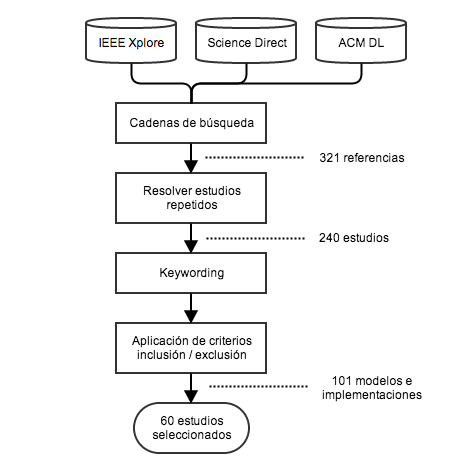
\includegraphics[width=0.7\textwidth]{figura-pasos}
	\caption{Pasos del mapeo sistemático realizado}
	\label{fig:pasos}
\end{figure}
\bigskip

La información fue extraída usando las herramientas de exportación de cada 
una de las bibliotecas digitales puesto
que ScienceDirect exporta a BibTex, IEEEXplore exporta a CSV. 
En el caso de ACM Digital Library se tuvo que usar una herramienta 
programada en PHP que recolectara la información automáticamente.

Después de eliminar los estudios que estaban doblemente
indexados, se comenzó con la etapa de \textit{keywording} y filtrado de
estudios según criterios. El \textit{keywording} se realizó leyendo los abstracts y etiquetando las
publicaciones según corresponda. Se iteró 2 veces para verificar que el 
criterio de etiquetado sea uniforme. Luego, se aplicaron los criterios de inclusión
y exclusión, en esta etapa se iteró varias veces para afinar el tamaño del conjunto
final del mapeo.


\begin{table}[h!]
\centering
\caption{Ejecución de cadenas de búsqueda en motores}
\label{tab:ejecucion-cadenas}
\begin{tabularx}{\textwidth}{p{3cm} X c} 
\toprule[1.5pt]
\bf	Motor		& \bf  Cadena	& 	\bf Resultado \\ \hline
ACM DL			& (Abstract:``electronic voting'' OR Abstract:``e-vote'') AND 
				(Abstract:``model'' OR Abstract:``scheme'' OR Abstract:``proposal'' 
				OR Abstract:``protocol'')										&	173	\\
				
IEEEXplore		&  (( Abstract:``electronic voting'' OR Abstract:``e-vote'') AND 
				(Abstract:``model'' OR Abstract:``scheme'' OR Abstract:``proposal'' 
				OR Abstract:``protocol''))										&	102	\\
ScienceDirect		& TITLE-ABSTR-KEY((``electronic voting'' OR ``e-vote'') AND (``model'' OR ``scheme'' OR ``proposal'' 
				OR ``protocol''))											&	46 	\\			
\bottomrule[0.5pt]
\end {tabularx}
\end{table}
\bigskip



\section{Esquema de clasificación}

Las publicaciones son clasificadas en 3 dimensiones: temporal, 
subcaracterísticas de calidad y tipo de propuesta. La estructura
es adaptada del trabajo de \cite{Petersen2007}. Estableciendo este 
esquema y la construcción del mapa fue hecho de manera iterativa
en cuanto al análisis de los trabajos fue modificado de acuerdo a las
sugerencias del profesor guía. 

\begin{itemize}
	\item La dimensión temporal se clasifica los trabajos de acuerdo al año de 
		publicación, tomando en cuenta sólo los últimos 10 años, de 2003 a 2010.
		
	\item La dimensión de subcaracterísticas de calidad clasifica los trabajos de acuerdo 
		a cual de las subcaracterísticas descritas en el estándar ISO/IEC 25010:2011 
		se enfoca el estudio. Se eligieron 8 subcaracterísticas  Hay publicaciones que pueden
		ser clasificadas en más de una subcaracterística, para resolver este problema 
		se construyeron categorías a partir de la combinación de las subcaracterísticas, 
		tal cual se ha visto en trabajos similares. \cite{Afzal}		
			
	\item La dimensión de tipo de propuesta clasifica las publicaciones en 4 tipos:
	\begin{itemize}
		\item  \textit{Solución criptográfica} aquellos trabajos que se limitan a 
			plantear soluciones a problemas detectados en otros 
			modelos centrados en criptografía. Aquí se incluyen trabajos que
			hayan realizado auditorías a otros modelos, hayan encontrado falencias y
			propongan mejoras. 
			
		\item   \textit{Propuesta criptográfica} trabajos que se limitan a plantear 
			o mejorar métodos criptográficos para una o varias funciones 
			de los sistemas de votación electrónica. Aquí se incluyen trabajos que
			sólo se limiten a presentar modelos que satisfagan los requisitos 
			básicos de la votación electrónica mediante
			la construcción de protocolos o esquemas criptográficos. Usualmente 
			son algoritmos basados en blind signature, homomorfic functions o mixnet.
			
		\item  \textit{Modelo} trabajos que plantean modelos generales de sistemas de 
			votación electrónica,que pueden utilizar uno o mas métodos criptográficos
			para realizar su función, o que proponen no sólo un algoritmo criptográfico
			sino también presenta revisiones y comparaciones con otros modelos, o que
			aborde otras funciones dentro del proceso eleccionario.
			
		\item  \textit{Implementacion} trabajos que describen a sistemas, o parte de estos,
			 ya construidos o relatan experiencias en la puesta en marcha de éstos. Aquí
			se incluyen trabajos que además de plantear un modelo, describen temas
			asociados a su implementación.
			
	\end{itemize}
	
\end{itemize}






